\section{Introduction}
\label{sec:introduction}

% Introduce the main tech of MEC, task offloading, add reference.
With the development of various mission-critical applications of Internet of Things (IoT), e.g. vehicular networks (both vehicle-to-vehicle and vehicle-to-infrastructure), augmented reality and city sensing, there is a need to ensure sufficient computational capacity and low latency connectivity is available for devices that are used in such applications. However, there is a tension between having sufficient computing resource and low latency in IoT applications. A cloud platform can have sufficient computing resources, however transferring data from IoT devices to cloud-based systems may introduce significant delay. This is particularly true in closer proximity to IoT devices, where the first hop network from the IoT device may have limited network capacity. A Mobile Edge Computing (MEC) framework is proposed to address some the above issues by offloading computation from IoT devices to local/ regional MEC servers instead of using a remote cloud system. This overcomes a number of potential constraints in current systems: lower energy consumption at the terminal devices\cite{mach2017mobile}, reduced requirement to transfer security-sensitive data to a cloud platform, and the need for network capacity between the IoT device and the cloud platform (over a multi-hop connection). 

Many existing offloading strategies for MEC environments focus on maximizing applications' performance by partitioning computational tasks across  IoT devices, MEC servers, and a cloud platform. However, there is limited coverage on development of the MEC network itself -- which is often assumed to be made of homogeneous types of devices/ resources. In rural environments and emergency relief scenarios, for example, the number of MEC servers are very limited. As a result, not all IoT devices can be covered by the MEC network. Inspired by~\cite{chen2017caching,zeng2016wireless,jeong2017mobile} that use drones (Unmanned Aerial Vehicles (UAVs)) to cache data generated from IoT devices that cannot be reached by cellular networks, we also describe the use of drones to forward cached data from IoT devices to MEC servers, rather than a  cloud platform.  The aim is to reduce the latency of data transmission via cellular networks.  

In addition, MEC server may be owned and operated by various organizations (e.g. Huawei, Google, Microsoft) and these providers need to work collaboratively to offer the ``best'' service to their costumers. This also raises a significant challenge of how to improve the visibility of the MEC service providers for handling users' sensitive data, or ensure some standard security and privacy requirements such as General Data Protection Regulation (GDPR) are met.  To achieve this, we use a blockchain network to improve the visibility of MEC service providers, helping increase trust from their customers. Moreover, we choose a permissioned, private blockchain to meet two essential requirements of our system: (i) offloading of tasks to the ``best" MEC server; (ii) developing a non-modifiable audit trail of which MEC server has been involved in processing user data (identifying ownership and processing carried by the MEC server). 

In this paper, we present a new secure offloading system that utilizes drones to extend the coverage of MEC networks and a private Blockchain is used to ensure the visibility and accountability of the MEC server providers on operating users' data while guaranteeing the performance of each offloading task. The proposed system has the following advantages:

% To tackle the above issues of task offloading in MEC scenarios, we present a high reliable architecture with drones based on the smart contract, shown in Figure \ref{fig:network-arch}, which brings the following advantages to offload tasks in MEC scenarios.

\begin{itemize}
\item \textbf{Cost efficiency \& accessibility}:
Using drones to cache data from IoT devices, and forwarding this to a MEC network that cannot be directly reached from the IoT device. This saves cost to deploy MEC servers, while ensuring coverage of MEC services.  
\item \textbf{Trustworthiness}:
The private blockchain only allows a certain members to participate in a pre-identified, permissioned network and the participants must follow restrictions or policies in the network. This can filter the untrustworthy MEC service provider.
\item \textbf{Visibility}: Blockchain is a decentralized system that secure data based on its completely transparent and verifiable property. Thus, in our proposed system, all the operations performed to users' data are recorded and can be verified, including which drone cached the data, which MEC server processed the data and what kind of analytic tasks are performed etc. 
% \item \textbf{Scalability}:
% The drone can make an authentication for each join or leave request from IoT devices. 
% Therefore, our architecture allows dynamic scale of IoT devices to access the offloading system by drones as the offloading hub.
 
% \item \textbf{Adaptivity}:
% The IoT device can modify the offloading policy according to its current requirement in real time by adopting Smart Contract, without negotiating with other nodes.
% % \item \textbf{Lightweight}:
% Our design avoids bringing IoT devices into blockchain network, thus the resource-constrained IoT devices can access to our architecture without any modification of their hardware.
% Besides, the drones as offloading hub, only need to have the capacity of parallel processing for multiple concurrent offloading requests. 
\end{itemize}

% Highlight the contribution of this work
To the best of our knowledge, this is the first work to adopt the blockchain technology in the drone-aided MEC scenarios.
% Compared with the traditional offloading systems, the design of offloading policy in a smart contract can simplify all operations in blockchain network and reduce the communication overhead among IoT devices, drones and MEC servers, especial for the handover among different offloading policies.
The main intellectual contributions of this work are summarized as follows.

\begin{enumerate}
\item A new decentralized offloading architecture in Drone-aided MEC(DMEC) framework is designed to improve the coverage of MEC services.
\item A new smart contract is designed to integrate with offloading policy for DMEC framework to ensure the visibility of MEC service providers involved in processing customers' data.
\item Simulation results demonstrate the feasibility of the proposed architecture in practical DMEC scenarios.
\end{enumerate}


% Article organization
The remainder of this article is organized as follows. 
We review related work in \S \ref{sec:related_work}.
The system architecture is described in \S \ref{sec:arch}.
Next, we propose a new smart contract to interact with offloading policy in MEC scenarios in \S \ref{sec:sys}.
In \S \ref{sec:eva}, experimental results show the feasibility of our architecture.
We present a security analysis of our architecture in \S \ref{sec:security_analysis}.
Finally, we conclude this paper and look forward the future work.

% \begin{figure*}[t]
% \centering
% 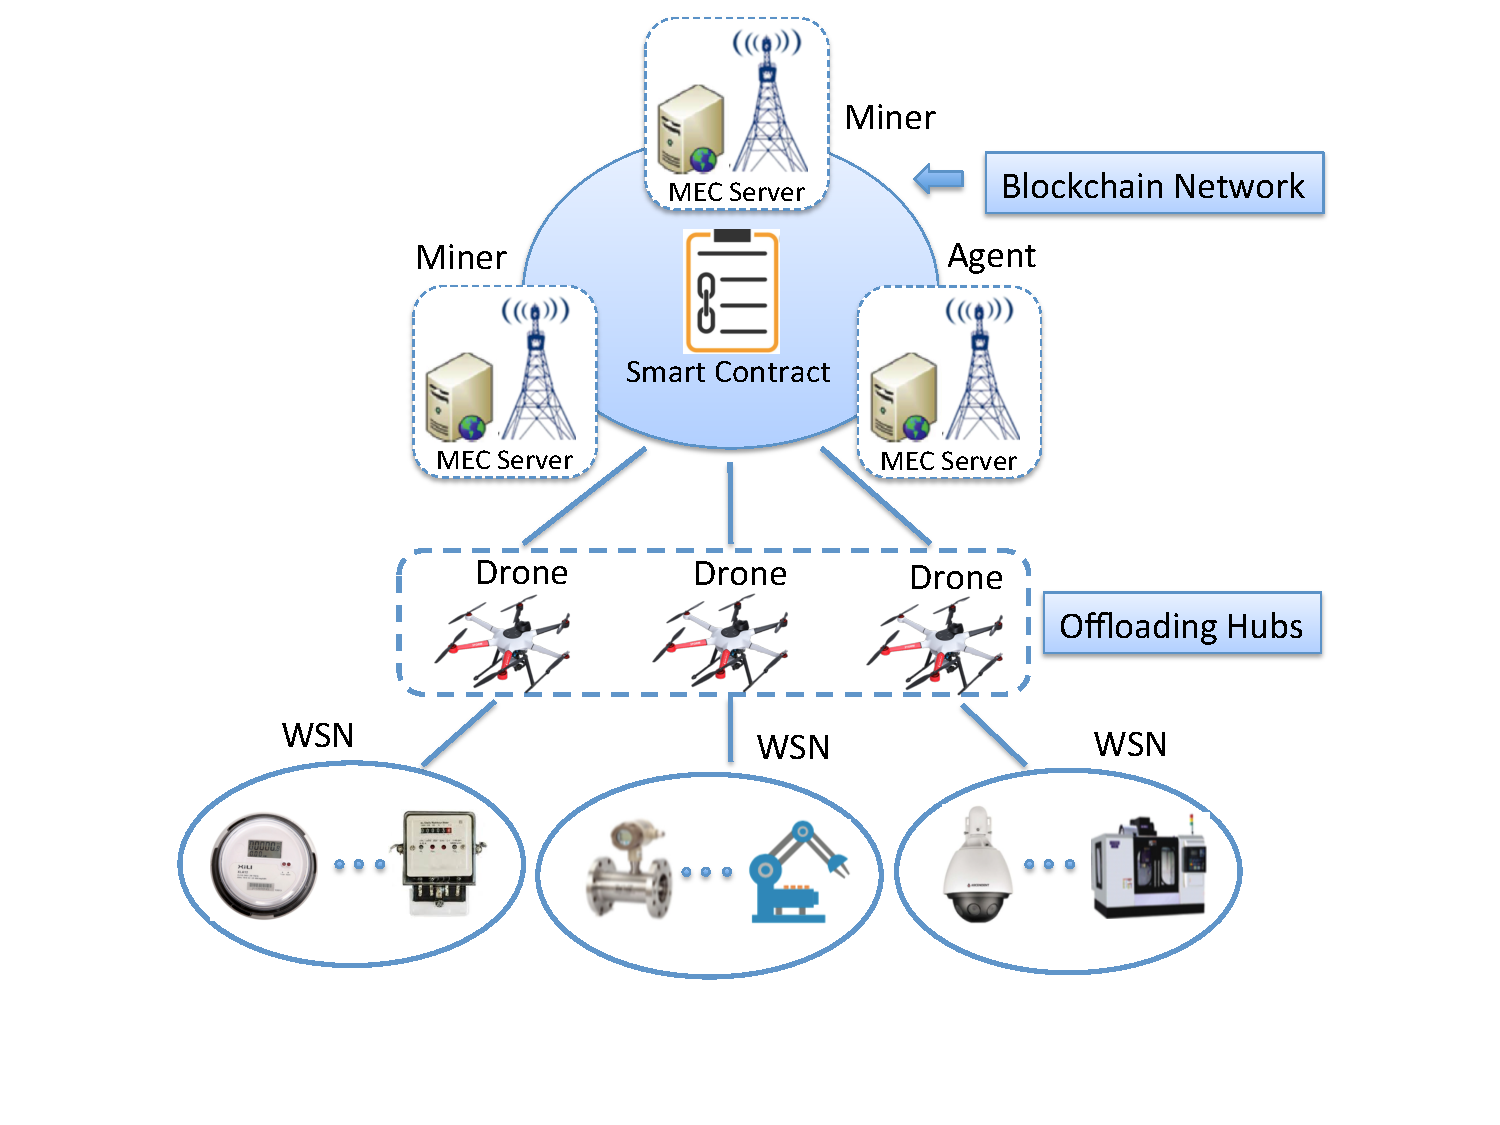
\includegraphics[width=3.5 in]{Fig/Architecture.pdf}
% \caption{Decentralized Offloading System}
% \label{fig:network-arch}
% \vspace*{-0.5\baselineskip}
% \end{figure*}



\begin{figure*}[t]
\centering
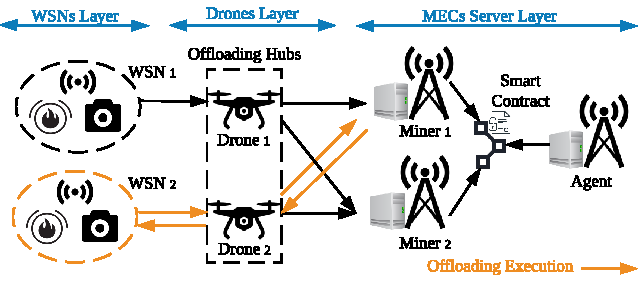
\includegraphics[width=5 in]{Fig/Architecture_1.pdf}
\caption{Decentralized Offloading System}
\label{fig:network-arch}
\vspace*{-0.5\baselineskip}
\end{figure*}

